\chapter{Auswertung}\label{text:Auswertung}

In den bisherigen Kapiteln wurde die umfassende Entwicklung des Stellwerks detailliert beschrieben. Ein besonderer Fokus lag auf der Implementierung der Fahrstraßenlogik sowie der konzeptionellen Entwicklung des Signaldecoders und des Weichendecoders. Dieses Kapitel zielt darauf ab, eine gründliche Untersuchung der Funktionalität dieser Schlüsselkomponenten durchzuführen. Durch gezielte Tests werden die Ergebnisse systematisch ausgewertet, um die Leistungsfähigkeit und Zuverlässigkeit des entwickelten Systems zu bewerten.

\section{Probleme}\label{text:Auswertung:Probleme}

In \autoref{text:Entwicklung-des-Stellwerks:Probleme-bei-der-Kommunikation} wurde auf \nameref{text:Entwicklung-des-Stellwerks:Probleme-bei-der-Kommunikation} zwischen den Modulen des Stellwerks eingegangen. Trotz intensiver Bemühungen konnten diese Herausforderungen bis zum Abschluss der Arbeit nicht zufriedenstellend gelöst werden. Die Schwierigkeiten in der Kommunikation zwischen den Komponenten verhinderten eine erfolgreiche Implementierung sowohl des Signal- als auch des Weichendecoders. Die exakte Ursache der Kommunikationsprobleme blieb unklar, was eine erhebliche Hürde für die weitere Entwicklung darstellte. Aufgrund dieser Problematik war es unmöglich, eine Gesamtprüfung der Stellwerksfunktionalität vorzunehmen, was die Validierung des Systems in seiner beabsichtigten Betriebsumgebung ausschloss. Stattdessen wurden die einzelnen Komponenten des Stellwerks getrennt getestet, um zumindest eine begrenzte Bewertung ihrer Funktionalität zu ermöglichen. Die Ergebnisse dieser Tests werden in den folgenden Abschnitten detailliert beschrieben.
\newline
Die Schwierigkeiten bei der Kommunikation waren allerdings nicht das einzige Hindernis bei der Entwicklung des Stellwerks. Durch die Wahl von Raspberry Pi Picos als Mikrocontroller musste das Projekt in Python oder C umgesetzt werden. Da C die deutlich bessere Performance bietet, wurde diese Sprache gewählt. Allerdings war die Entwicklung in C für das Team eine große Herausforderung, da es für viele Anwendungsfälle weder Erfahrung noch gute Dokumentation anderer Bibliotheken gab. Dies führte zu einer langsameren Entwicklung, Verstädnisproblemen und mehr Fehlern, die behoben werden mussten. Ein weiteres Problem war die mangelnde Erfahrung des Teams mit der Entwicklung von Hardware und die damit verbundenen Schwierigkeiten bei der Fehlersuche. Als Beispiel sei hier die Fehlersuche bei der Kommunikation zwischen den Modulen genannt. Da das Team keine Erfahrung mit der Kommunikation zwischen Mikrocontrollern hatte, war es schwierig, die Ursache des Problems zu finden. Dies führte zu einer längeren Entwicklungszeit und einer geringeren Qualität des Endprodukts.
\newpage
\section{Gleisfreimeldung}\label{text:Grundlagen:Gleisfreimeldung}

Die Gleisfreimeldung ist ein wichtiges Element der Sicherungstechnik im Schienenverkehr. Ihre scheinbar einfache Aufgabe ist es, das Frei- oder Besetztsein eines Gleisabschnittes zu überwachen und dem Stellwerk zu melden. Heutzutage sind zwei verschiedene Arten der Gleisfreimeldung im Einsatz: Gleisstromkreise und Achszähler. In diesem Abschnitt werden nach einer Betrachtung der Historie, beide Systeme vorgestellt und ihre Funktionsweise erläutert.

\subsection{Historische Gleisfreimeldung}\label{text:Grundlagen:Gleisfreimeldung:Historische-Gleisfreimeldung}

\subsection{Gleisstromkreis}\label{text:Grundlagen:Gleisfreimeldung:Gleisstromkreis}

Gleisstromkreise bestimmen den Belegungszustand eines Freimeldeabschnitts über Stromkreise, die durch die Räder der Schienenfahrzeuge geschlossen werden.~\cite[][S. 47]{bib:Sicherung-des-Schienenverkehrs} \autoref{abb:Grundlagen:Gleisfreimeldung:Gleisstromkreis} zeigt den Aufbau eines Gleisstromkreises.

\begin{figure}[H]
    \centering
    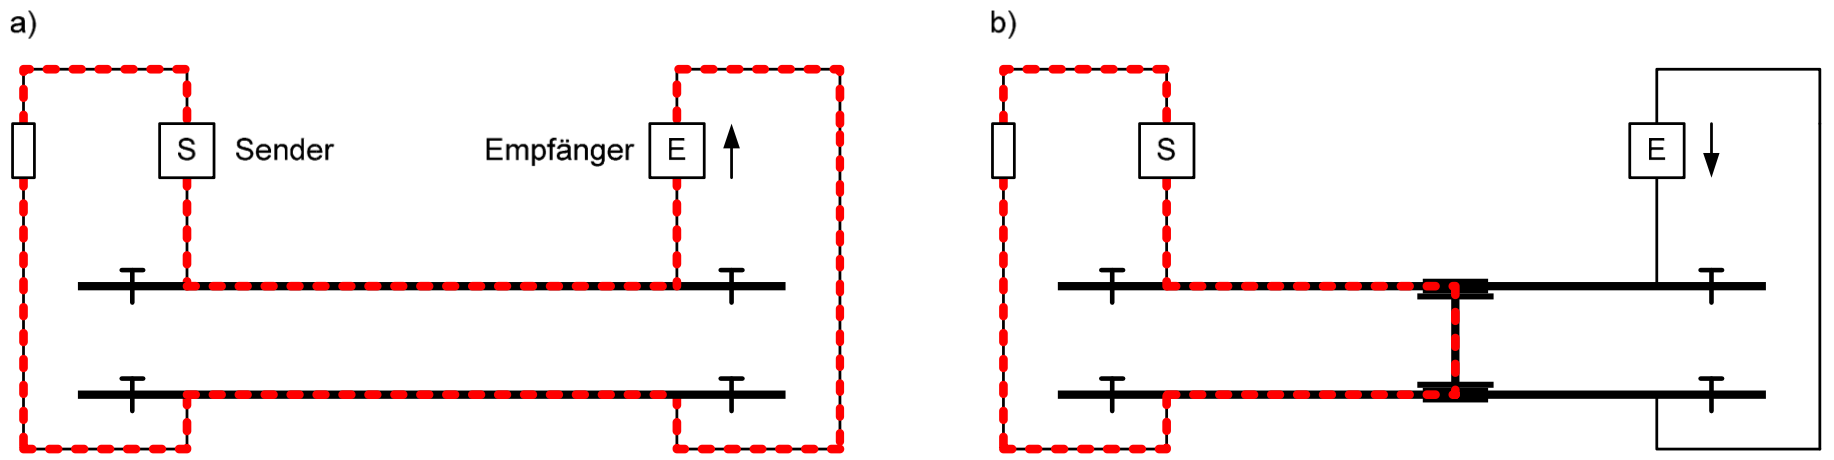
\includegraphics[width=0.7\textwidth]{Assets/Images/2-Grundlagen/Gleisstromkreis.png}
    \caption{Aufbau eines Gleisstromkreises~\cite[][S. 47]{bib:Sicherung-des-Schienenverkehrs}}\label{abb:Grundlagen:Gleisfreimeldung:Gleisstromkreis}
\end{figure}

\textquote{Gleisstromkreise arbeiten nach dem Ruhestromprinzip. Dabei liegt in Grundstellung (freies Gleis) ein geschlossener Stromkreis vor.}~\cite[][S. 47]{bib:Sicherung-des-Schienenverkehrs} Wird ein Gleisabschnitt durch ein Schienenfahrzeug belegt, wird der Stromkreis unterbrochen. Die Unterbrechung des Stromkreises wird vom Stellwerk registriert und als belegt gemeldet.~\cite[][S. 47]{bib:Sicherung-des-Schienenverkehrs} Befindet sich eine Achse im Gleisfreimeldeabschnitt, so wird der Stromkreis geschlossen und der Abschnitt dem Stellwerk besetzt gemeldet.~\cite[][S. 47]{bib:Sicherung-des-Schienenverkehrs}

Ein großer Vorteil von Gleisstromkreisen ist, dass sie in der Lage sind auch stehende Fahrzeuge zu erkennen. Allerdings kann es bei Störungen der Leitfähigkeit der Schienen zu Fehlmeldungen kommen.

\subsection{Achszähler}\label{text:Grundlagen:Gleisfreimeldung:Achszähler}

Achszähler bestimmen den Belegungszustand eines Freimeldeabschnitts über die Zählung der ein- und ausfahrenden Achsen.~\cite[][S. 53]{bib:Sicherung-des-Schienenverkehrs} \autoref{abb:Grundlagen:Gleisfreimeldung:Achszaehlkreis} zeigt den Aufbau eines Achszählkreises.

\begin{figure}[H]
    \centering
    \includegraphics[width=0.7\textwidth]{Assets/Images/2-Grundlagen/Achszählkreis.png}
    \caption{Aufbau eines Achszählkreises~\cite[][S. 53]{bib:Sicherung-des-Schienenverkehrs}}\label{abb:Grundlagen:Gleisfreimeldung:Achszaehlkreis}
\end{figure}

Am Gleis sind Elektromagnete (Schienenkontakte), angebracht, deren Magnetfeld bei Überfahrt eines Rades gestört wird. Diese Störung wird registriert und die Achse gezählt. Achszähler sind in der Lage, die Fahrtrichtung zu bestimmen, indem zwei nah beieinander liegende Schienenkontakte verbaut werden.~\cite[][S. 53 ff.]{bib:Sicherung-des-Schienenverkehrs} \autoref{abb:Grundlagen:Gleisfreimeldung:Doppelter-Schienenkontakt} zeigt einen solchen doppelten Schienenkontakt.

\begin{figure}[H]
    \centering
    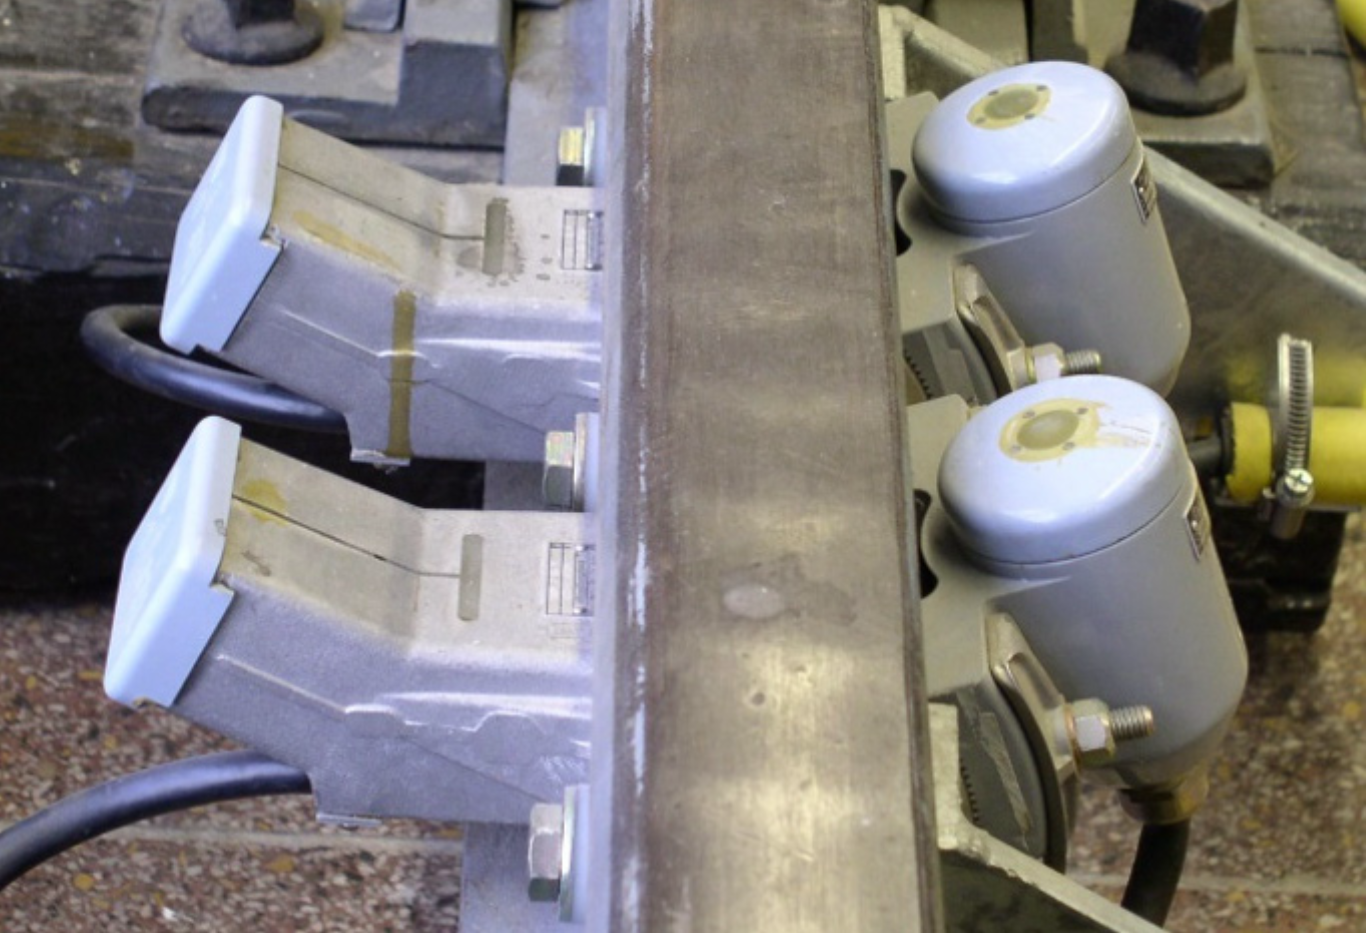
\includegraphics[width=0.7\textwidth]{Assets/Images/2-Grundlagen/Doppelter-Schienenkontakt.png}
    \caption{Doppelter Schienenkontakt~\cite[][S. 54]{bib:Sicherung-des-Schienenverkehrs}}\label{abb:Grundlagen:Gleisfreimeldung:Doppelter-Schienenkontakt}
\end{figure}

Im Gegensatz zu Gleisstromkreisen sind Achszähler nicht in der Lage stehende Fahrzeuge zu erkennen, können jedoch die Fahrtrichtung feststellen.

\newpage
\input{Text/6-Auswertung/Fahrstraßenlogik.tex}
\newpage